% Created 2018-06-21 Thu 12:30
\documentclass[8pt]{beamer}
\usepackage[sc,osf]{mathpazo}   % With old-style figures and real smallcaps.
\linespread{1.025}              % Palatino leads a little more leading
% Euler for math and numbers
\usepackage[euler-digits,small]{eulervm}
%\documentclass[10pt]{llncs}
%\usepackage{llncsdoc}
\usepackage{hyperref}
\usepackage{minted}
\usepackage[utf8]{inputenc}
\usepackage[T1]{fontenc}
\usepackage{fixltx2e}
\usepackage{graphicx}
\usepackage{longtable}
\usepackage{float}
\usepackage{wrapfig}
\usepackage{rotating}
\usepackage[normalem]{ulem}
\usepackage{amsmath}
\usepackage{textcomp}
\usepackage{marvosym}
\usepackage{wasysym}
\usepackage{amssymb}
\usepackage{polynom}

\hypersetup{colorlinks=true,
    linkcolor = blue,
    urlcolor  = blue,
    citecolor = blue,
    anchorcolor = blue
}
\renewcommand{\mod}[1]{\left( \texttt{mod}~#1 \right)}
\newcommand{\N}{\mathbb N}
\newcommand{\B}{\mathbb B}
\newcommand{\Z}{\mathbb Z}
\newcommand{\Q}{\mathbb Q}
\newcommand{\C}{\mathbb C}
\newcommand{\degree}{\texttt{degree}}
\newcommand{\cpp}[1]{\mintinline{cpp}{#1}}
\newcommand{\py}[1]{\mintinline{py}{#1}}
\newcommand{\raw}[1]{\mintinline{text}{#1}}
\newcommand{\hs}[1]{\mintinline{hs}{#1}}
\tolerance=1000
\usetheme{Antibes}
% \usetheme{Warsaw}
\author{Siddharth Bhat}
\date{October 18th, 2019}
\institute{IIIT Open Source Developers group}
\title{A taste of Haskell?}
\hypersetup{
  pdfkeywords={},
  pdfsubject={},
  pdfcreator={Emacs 24.5.1 (Org mode 8.2.10)}}
\begin{document}

\maketitle

\begin{frame}[fragile]{What's programming like?}
    A lot like building a cathedral.
    \pause
    \begin{columns}
    \column{0.5\textwidth}
    \begin{figure}
    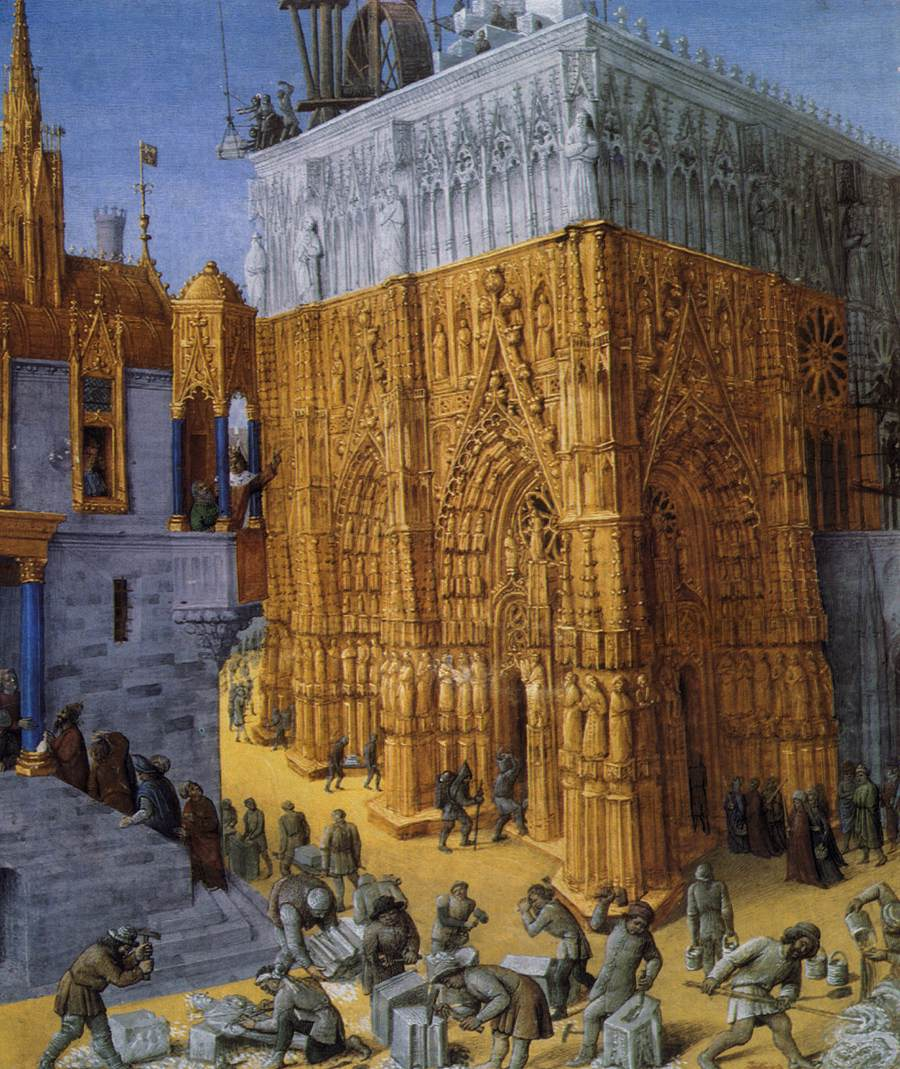
\includegraphics[height=5cm]{./first-we-build.jpg}
    \caption{First we build}
    \end{figure}
    \column{0.5\textwidth}
    \pause
    \begin{figure}
    
\includegraphics[height=5cm]{./then-we-pray.jpg}
    \caption{Then we pray}
    \end{figure}
    \end{columns}
\end{frame}

\begin{frame}[fragile]{Why we pray}
\pause

{\small
\begin{minted}{cpp}
#include <iostream>
#include <climits>
using namespace std;

// f(x) == true ?
bool f(unsigned x) { return (x + 1) > x; }

int main() {
    cout << "f(0): " << f(0) << "\n";
    cout << "f(UINT32_MAX: " << f(UINT32_MAX) << "\n";
}
\end{minted}
}

\pause
\begin{minted}{text}
f(0): 1
f(UINT32_MAX):0
\end{minted}

\pause
\begin{itemize}
    \item 
        $f: \N \rightarrow \B; f(x) \equiv \begin{cases} \texttt{true} & x + 1 > x \\ \texttt{false} & \text{otherwise} \end{cases}$
        \pause
    \item $f(x) \equiv \texttt{true}$ \pause
    \item $f: \N \rightarrow \B; f(x) \equiv \begin{cases} \texttt{true} & x +_{2^{32}} 1 > x \\ \texttt{false} & \text{otherwise} \end{cases}$ \pause
    \item $+_{2^32}: \N \times \N \rightarrow \N; x +_{2^{32}} y \equiv (x +_\N y) \% 2^{32}$ \pause 
    \item $\texttt{UINT32\_MAX} +_{2^{32}} 1 = 0 $
\end{itemize}
\end{frame}


\begin{frame}[fragile]{Why we pray: A second example}
\begin{minted}{cpp}
int main() {
  cout << 2 * ((int) getchar()) << "\n";
}
\end{minted}
\pause

$$ \forall x \in \Z, 2 * x = x + x$$
\pause

\begin{minted}{cpp}
int main() {
  cout << ((int)getchar() + (int)getchar()) << "\n";
}
\end{minted}

\pause


\begin{itemize}
    \item \cpp{int getchar()} \pause
    \item $\texttt{getchar}: \emptyset \rightarrow \texttt{int}$ \pause
    \item $\{ \} \rightarrow \{ 1, 42, \dots \}$ \pause
    \item Such a function can't return an output! \pause
    \item $\texttt{getchar}: \{ \star \} \rightarrow \texttt{int}$ \pause
    \item $\{ \star \} \rightarrow \{ 1, 42, \dots \}$ \pause
    \item $\{ \star \} \rightarrow \{ 1, 42, \dots \}~ \star \mapsto 42$ \pause
    \item Such a function will always return the same output! \pause
    \item \texttt{getchar} can't be a mathematical function.
\end{itemize}

\pause

\end{frame}

\begin{frame}[fragile]{Why we pray: A third example}
\begin{minted}{cpp}
int K (int x, int y) { return x; } // K(x, y) = x
\end{minted}
\pause
\begin{minted}{cpp}
int main() { cout << K(10, 20) << "\n" cout << 10; }
\end{minted}
\pause
\cpp{K(10, 20)} $=  10$
\pause
\begin{minted}{cpp}
int err() { exit(1); return 0; }
int main() { cout << K(10, err()) << "\n" cout << 10; }
\end{minted}
\pause
\cpp{K(10, err())} $\neq 10$
\pause

\begin{itemize}
    \item Mathematically, can replace $K(x, y)$ by $x$. \pause
    \item In C(++), impossible. \pause
    \item cannot \textbf{equationally reason} about programs. \pause
    \item \textbf{Can we} reason about programs? \pause
\end{itemize}
\end{frame}

\begin{frame}[fragile]{Can we reason about C++?}
    \pause
    \begin{itemize}
    \item Short answer: Yes. \pause
    \item Longer answer: Yes. It's complicated. \pause
    \item Name dropping: Operational/Denotational semantics. \pause
    \item Name dropping: Hoare logic/Separation logic. \pause
    \end{itemize}
\end{frame}


\begin{frame}[fragile]{How do we escape having to pray?}
    \pause
    Define a language, \pause where anything that happens, \pause is what \textbf{mathematics} says should happen.
    \pause

\begin{figure}

\includegraphics[height=1cm]{./haskell-logo.png}
\end{figure}
\end{frame}

\begin{frame}[fragile]{A taste of Haskell}
    \begin{itemize}
        \item \hs{let xs = [1, 2,..10]} \pause
        \item \py{xs = range(10)} \pause
        \item \hs{let nats = [1, 2..]} \pause
        \item \py{xs = ??} \pause
        \item \item \hs{take 2 nats} \pause
        \item \item \hs{take 10 nats} \pause
        \item \item \hs{take 100 nats} \pause
    \end{itemize}
\end{frame}

\begin{frame}[fragile]{Philosophical differences}

{\tiny \url{docs.python.org/3/library/stdtypes.html#str.join}}
{\tiny \url{hackage.haskell.org/package/base-4.14.0.0/docs/Data-List.html#v:intercalate}}

\begin{columns}% [T] % align columns
\begin{column}{.48\textwidth}
\begin{minted}{py}
" ".join(["a", "b", "c", "d"])
\end{minted}
\begin{minted}{text}
str.join(iterable)
\end{minted}

Return a string which is the concatenation of the strings in \emph{iterable}. A
\verb|TypeError| will be raised if there are any non-string values in \emph{iterable},
including \verb|bytes objects|. The separator between elements is the string providing
this method.


\end{column}
%
\begin{column}{.48\textwidth}
\begin{minted}{hs}
intercalate " " ["a", "b", "c", "d"]
\end{minted}

\begin{minted}{hs}
intercalate :: [a] -> [[a]] -> [a]
\end{minted}

\verb|intercalate xs xss| is equivalent to \verb|(concat (intersperse xs xss))|.
It inserts the list \verb|xs| in between the lists in \verb|xss| and concatenates the result.

\end{column}
\end{columns}

\end{frame}

\begin{frame}[fragile]{Why should I learn haskell?}

{\tiny \url{https://docs.python.org/3/library/functions.html#sum}}
{\tiny \url{hackage.haskell.org/package/base-4.14.0.0/docs/Data-List.html#v:intercalate}}

\begin{columns}% [T] % align columns
\begin{column}{.48\textwidth}
\begin{minted}{py}
sum([1, 2, 3, 4])
\end{minted}
\begin{minted}{text}
sum(iterable, /, start=0)
\end{minted}

Sums \emph{start} and the items of an \emph{iterable} from left to right and
returns the total. The \emph{iterable}’s items are normally numbers, and the start
value is not allowed to be a string.


\end{column}
%
\begin{column}{.48\textwidth}
\begin{minted}{hs}
sum [1, 2, 3, 4]
\end{minted}

\begin{minted}{hs}
sum :: (Foldable t, Num a) => t a -> a
\end{minted}

The \verb|sum| function computes the sum of the numbers of a structure.

\end{column}
\end{columns}
\end{frame}

\begin{frame}[fragile]{\texttt{Foldable} in detail}


\begin{minted}{hs}
class Foldable t where
  -- | Map each element of the structure to a monoid, and combine the results.
  foldMap :: Monoid m => (a -> m) -> t a -> m
\end{minted}

\verb|Foldable| instances are expected to satisfy the following laws:

\begin{minted}{hs}
foldr f z t = appEndo (foldMap (Endo . f) t ) z
foldl f z t = appEndo (getDual (foldMap (Dual . Endo . flip f) t)) z
fold = foldMap id
length = getSum . foldMap (Sum . const  1)
\end{minted}
{\tiny \url{https://hackage.haskell.org/package/base-4.14.0.0/docs/Data-Foldable.html#t:Foldable}}
\end{frame}


\begin{frame}[fragile]{Fibonacci}
\begin{minted}{hs}
let fib = 0:1:(zipWith (+) fib (tail fib))
\end{minted}
\end{frame}


\begin{frame}[fragile]{Equational reasoning}
\begin{minted}{hs}
k x y = x
k 10 (error "urk")
\end{minted}


\begin{minted}{py}
def k(x, y): return x
k(x, input())
\end{minted}
\end{frame}


\begin{frame}[fragile]{What is \texttt{input} anyway?}
$$\emptyset \mapsto \texttt{char} $$
Mathematically impossible!
\end{frame}

\begin{frame}[fragile]{Effects, or the ``\texttt{M}'' word}
Keep every element, and drop every element.
\begin{minted}{hs}
powerset xs = filterM (const [True, False]) xs
\end{minted}
\end{frame}



\end{document}
